\documentclass[a4paper, 12pt]{article}
\usepackage[utf8]{inputenc}
\renewcommand\familydefault{\sfdefault}
\usepackage[T1]{fontenc}
\usepackage[francais]{babel}
\usepackage[left=2.5cm,top=2.5cm,right=2.5cm,bottom=2.5cm]{geometry}
\usepackage{graphicx}
\usepackage[usenames, dvipsnames]{xcolor}
\definecolor{mygray}{gray}{0.95}

\usepackage{minted}
\usemintedstyle{colorful}
\usepackage{float}
\floatplacement{figure}{H}
\usepackage{authblk}
\usepackage{enumitem}
\usepackage{hyperref}
\hypersetup{
    colorlinks,
    citecolor=black,
    filecolor=black,
    linkcolor=black,
    urlcolor=blue
}

\usepackage{caption}
\newenvironment{code}{\captionsetup{type=listing}}{}
\usepackage{array}
\usepackage{etoolbox}
\patchcmd{\thebibliography}{\section*{\refname}}{}{}{}

\usepackage{dirtree}

\usepackage{glossaries}
	\let\oldnewacronym\newacronym
	\newcommand*{\provideacronym}[3]{%
	  \ifglsentryexists{#1}{%
	  }{%
	    \oldnewacronym{#1}{#2}{#3}%
	  }%
	}
\makeglossaries


\begin{document}

\title{Conception d'un système de "tagging" des fichiers avec Rust}
\author{Steven Liatti}
\affil{\small Projet de bachelor - Prof. Florent Glück}
\affil{\small Hepia ITI 3\up{ème} année}
\maketitle

\subparagraph{Résumé}
Le but de ce projet est de concevoir et développer un "moteur de gestion de tags" pouvant gérer des dizaines de milliers
de fichiers et tags associés de manière efficace, en Rust. Le stockage des tags utilisera le mécanisme des "extended
attributes" disponibles dans la plupart des systèmes de fichiers modernes. Le moteur d'indexation devra surveiller les
fichiers modifiés, créés, ou supprimés afin d'indexer les tags avec un minimum de latence (temps réel). Si le temps le
permet, le système développé sera intégré à un environnement desktop choisi (Gnome, KDE, etc.).

% \begin{figure}
% 	\begin{center}
% 		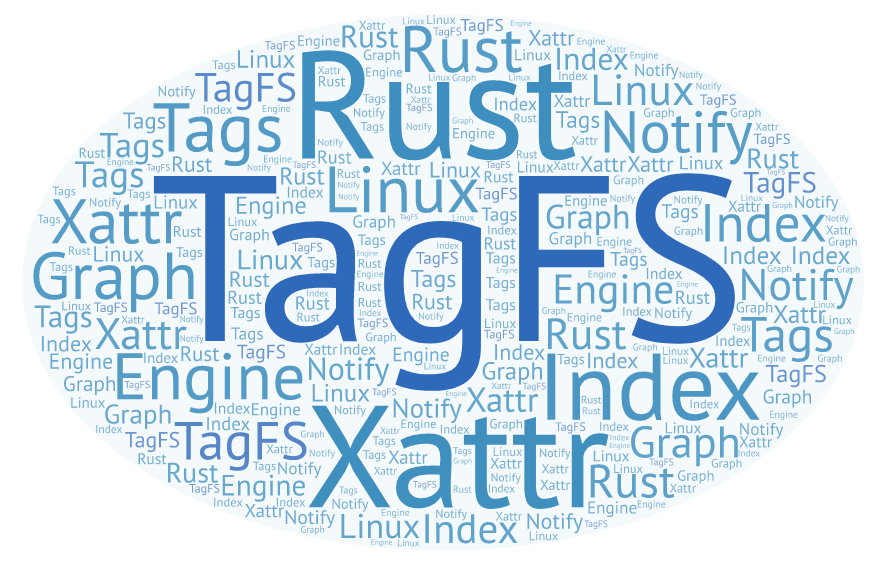
\includegraphics[width=0.43\textwidth]{images/title.png}
% 	\end{center}
% \end{figure}

\begin{figure}[!b]
	\centering
	\begin{minipage}{.4\textwidth}
		\centering
		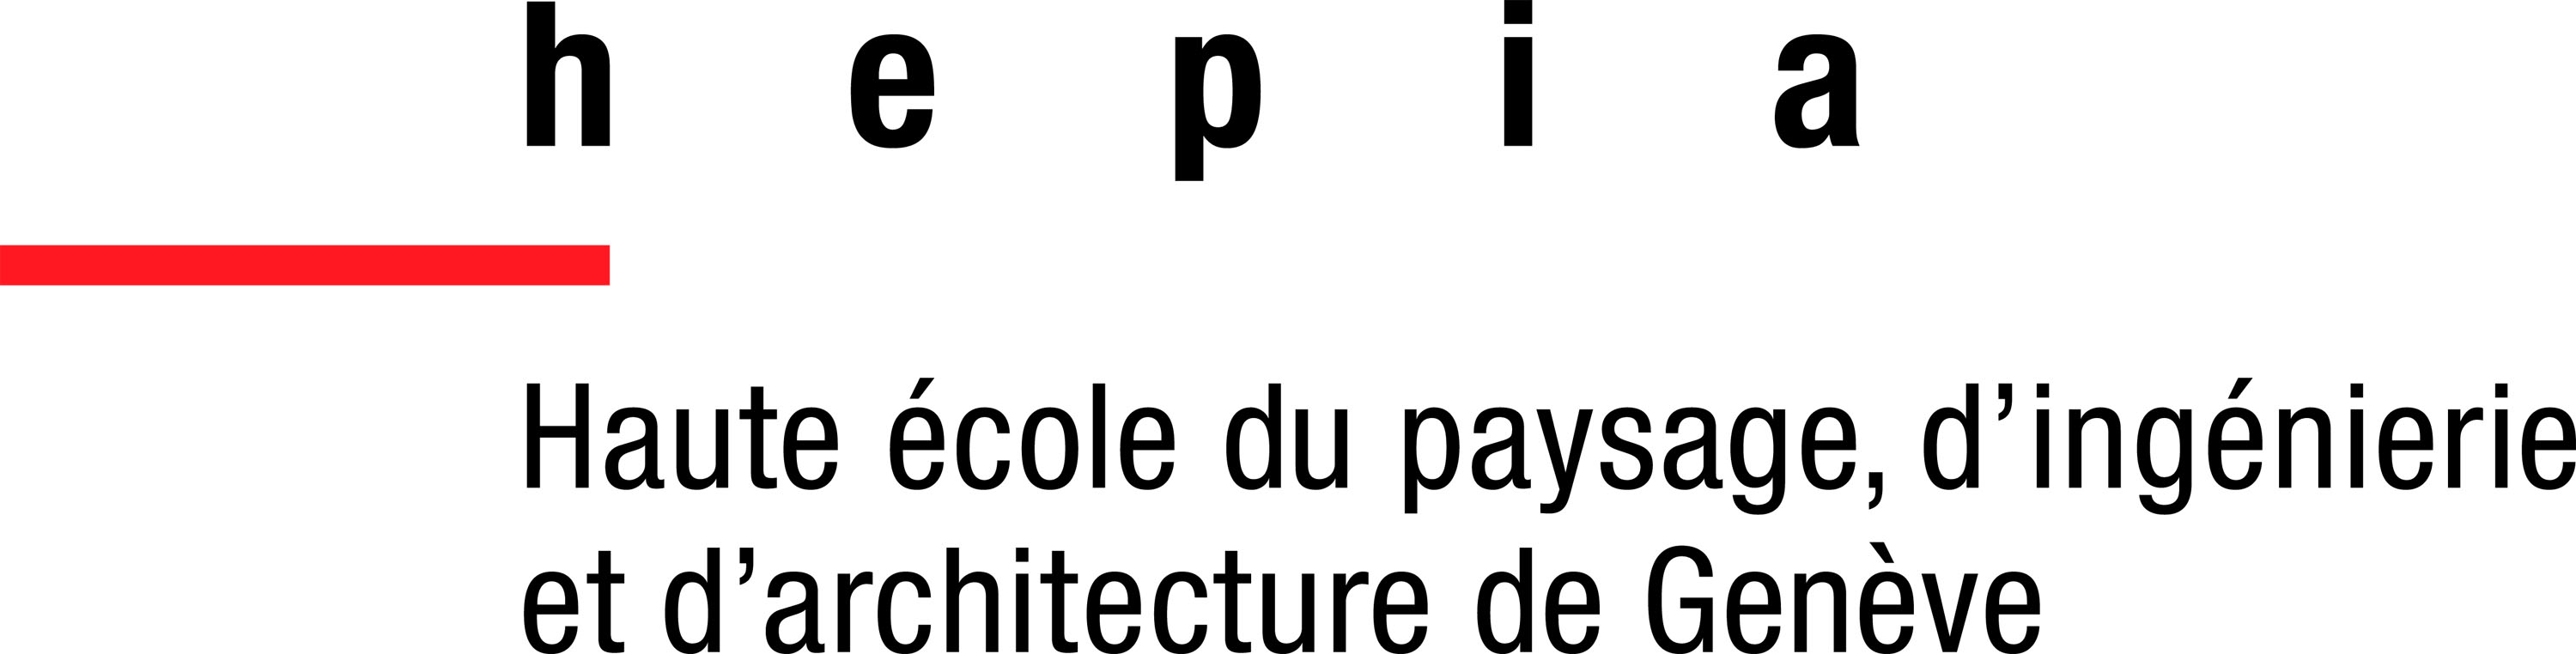
\includegraphics[width=.6\linewidth]{images/hepia.jpg}
	\end{minipage}%
	\begin{minipage}{.4\textwidth}
		\centering
		
\includegraphics[width=.6\linewidth]{images/hesso.jpg}
	\end{minipage}
\end{figure}
\newpage

\newpage

% \setcounter{tocdepth}{2}
\tableofcontents
\listoffigures
\renewcommand\listoflistingscaption{Table des listings de code source}
\listoflistings
\newpage

\section*{Conventions typographiques}
Lors de la rédaction de ce document, les conventions typographique ci-dessous ont
été adoptées.
\begin{itemize}[label=\textbullet]
	\item Tous les mots empruntés à la langue anglaise ont été écrits en \textit{italique}
	\item Toute référence à un nom de fichier (ou dossier), un chemin d'accès, une 
    utilisation de paramètre, variable, ou commande utilisable par l'utilisateur, 
    est écrite avec la police d'écriture \mintinline{text}{Courier New}.
	\item Tout extrait de fichier ou de code est écrit selon le format suivant:
    \bigbreak
    \begin{code}
        \begin{minted}[bgcolor=mygray,breaklines,breaksymbol=,linenos,frame=single,stepnumber=1,tabsize=2]{rust}
fn main() {
    println!("Hello, world!");
}
        \end{minted}
    \end{code}
\end{itemize}
\newpage

\newacronym{xattr}{XATTR}{\textit{Extended Attributes}}
\printglossary[type=\acronymtype,title={Acronymes}]
\newpage


\section{Introduction} %--------------------------------------------------
\acrshort{xattr}
\subsection{Motivations}
\subsection{Buts}
\cite{ref3}

\section{Analyse de l'existant} %--------------------------------------------------
Dans cette section, nous allons analyser les principales solutions existantes, qu'elles soient 
sous la forme d'applications utilisateur ou intégrées directement dans un système d'exploitation.
Jean-Francois Dockes en dresse également une liste avec avantages et inconvénients sur son site 
\cite{ref3}.

\subsection{Applications utilisateur}
\subsubsection{TMSU}
TMSU \cite{ref15} est un outil en ligne de commande (CLI) qui permet d'attribuer des tags à des 
fichiers et d'exécuter des recherches par tags. On commence par initialiser TMSU dans le dossier choisi. 
Une commande liste les tags associés à un ou 
plusieurs fichiers et une autre liste les fichiers qui possèdent le ou les tags donnés. TMSU offre 
la possibilité à l'utilisateur de "monter" un système de fichier virtuel avec FUSE (Filesystem in 
UserSpacE). L'outil est rapide et efficace, mais il comporte quelques défauts :
\begin{itemize}
    \item Pas d'interface graphique
    \item Dépendance à FUSE pour monter le système de fichiers virtuel
    \item Stockage des tags dans une base de données SQLite
\end{itemize}

\subsubsection{Tagsistant}
Tagsistant \cite{ref16} est autre outil CLI de gestion de tags. Il dépend de FUSE et d'une base 
de données (SQLite ou MySQL) pour fonctionner. Comme pour TMSU, il faut donner un dossier à Tagsistant 
pour son usage interne. À l'intérieur de ce dernier, se trouvent différents dossiers :
\dirtree{%
.1 /.
.2 alias --- Dossier contenant les requêtes les plus courantes.
.2 archive --- Dossier listant les fichiers.
.2 relations --- Dossier contenant les relations entre les tags et fichiers.
.2 stats --- Dossier contenant des infos sur l'utilisation de Tagsistant.
.2 store --- Dossier où sont taggés les fichiers.
.2 tags --- Dossier de gestion des tags.
}
\bigbreak
Chaque dossier a un rôle bien précis. Tout se fait avec le terminal et des commandes usuelles 
(\mintinline{text}{cp}, \mintinline{text}{ls}, \mintinline{text}{mkdir}, etc.). Dans Tagsistant, 
un dossier créé dans le dossier \mintinline{text}{tags} correspond à un tag. On se retrouve 
finalement avec une arborescence de tags et de fichiers \cite{ref17}. Bien que cet outil soit 
performant d'un point de vue de la rapidité d'exécution, il comporte les défauts de TMSU ainsi que 
des nouveaux :
\begin{itemize}
    \item Pas d'interface graphique
    \item Dépendance à FUSE pour monter le système de fichiers virtuel
    \item Stockage des tags dans une base de données
    \item Utilisation des différents dossiers peu intuitive
\end{itemize} 

\subsubsection{TaggedFrog}
TaggedFrog \cite{ref18} est un programme disponible sur Windows uniquement et ne partage pas ses sources.
Son fonctionnement interne n'est pas documenté. L'interface est agréable, on peut ajouter des fichiers 
par Drag \& Drop. L'interface créé au fur et à mesure un "nuage" de tags, comme on peut le retrouver sur 
certains sites web. On peut exécuter des recherches sur les tags et les fichiers. On peut supposer que 
TaggedFrog maintient une base de données des tags associés aux fichiers, ce qui ne correspond à nouveau 
pas à nos besoins.
\begin{figure}
    \begin{center}
        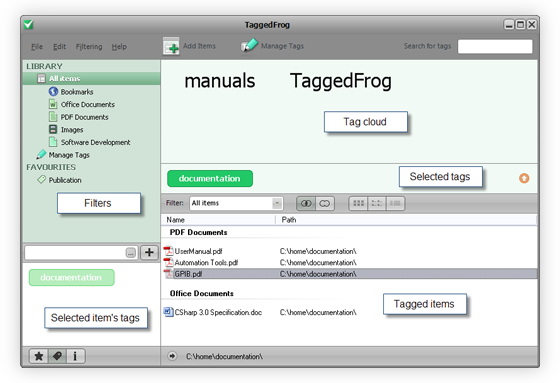
\includegraphics[width=0.8\textwidth]{images/taggedfrog.png}
    \end{center}
    \caption{TaggedFrog en utilisation \cite{ref18}}
    \label{taggedfrog}
\end{figure}

\subsubsection{TagSpaces}
TagSpaces \cite{ref13} est un programme avec une GUI permettant d'étiqueter ses fichiers avec des tags. 
L'application est agréable à utiliser, on commence par connecter un emplacement qui fera office de dossier de 
destination aux fichiers. On peut ajouter ou créer des fichiers depuis l'application. Les fichiers 
existants ajoutés depuis l'application sont copiés dans le dossier (cela créé donc un doublon). 
Sur le panneau de gauche se situe la zone de gestion des tags. TagSpaces ajoute automatiquement 
certains tags dits "intelligents" aux fichiers nouvellement créés avec l'application (par exemple 
un tag avec la date de création).
\begin{figure}
    \begin{center}
        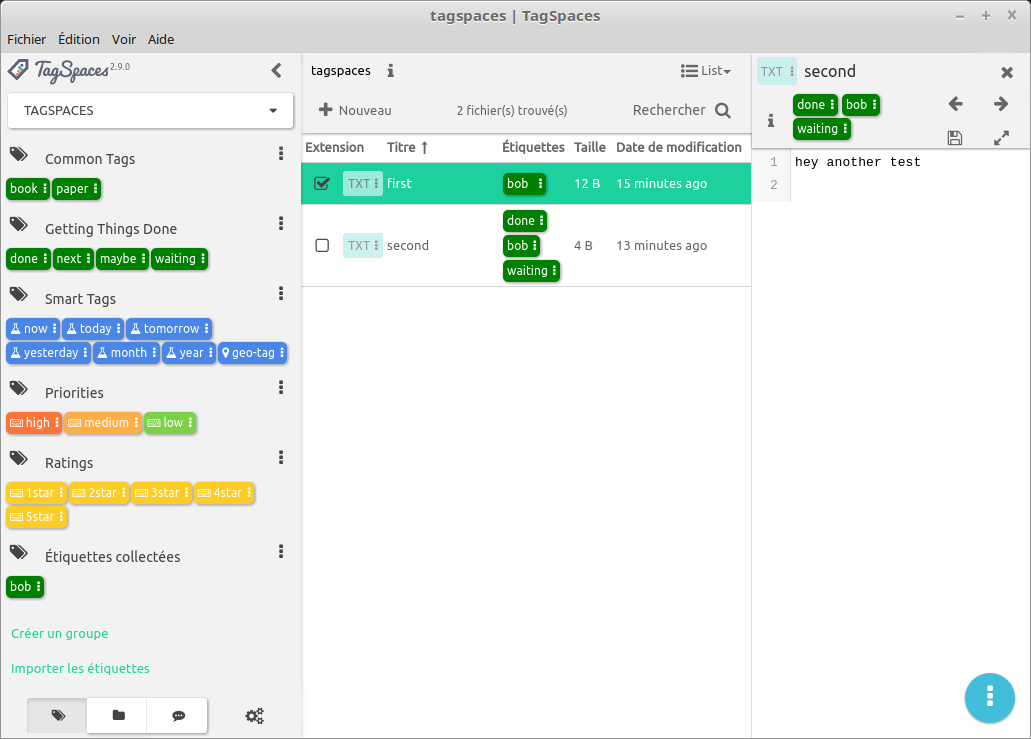
\includegraphics[width=0.8\textwidth]{images/tagspaces.png}
    \end{center}
    \caption{TagSpaces en utilisation}
    \label{tagspaces}
\end{figure}
Globalement, l'application est fonctionnelle et \textit{user friendly}. Cependant, 2 points noirs 
sont à déplorer :
\begin{enumerate}
    \item L'application copie les fichiers déjà existants sélectionnés par l'utilisateur, ce qui 
        créé une contrainte supplémentaire dans la gestion de ses fichiers personnels.
    \item TagSpaces stocke les tags directement dans le nom du fichier, modifiant ainsi son nom \cite{ref14}.
        Bien que pratique dans le cas d'une synchronisation à l'aide d'un service cloud, 
        le fichier devient dépendant de TagSpaces, si l'utilisateur décide de changer son nom sans 
        respecter la nomenclature interne, il risque de perdre les tags associés au fichier.
\end{enumerate}

\subsection{Fonctionnalités incluses dans le système d'exploitation}
% \subsubsection{BeOS}
% \subsubsection{Linux}

\subsubsection{Windows}
À partir de Windows Vista, Microsoft a donné la possibilité aux utilisateurs d'ajouter des 
méta-données aux fichiers; parmi ces méta-données se trouvent les tags. Il existe une fonctionnalité 
appelée \textit{Search Folder} qui permet de créer un dossier virtuel contenant le résultat d'une 
recherche sur les noms de fichiers ou d'autres critères \cite{ref19}. Depuis Windows 8, l'utilisateur 
a la possibilité d'ajouter des méta-données à certains types de fichiers (ceux de la suite office 
par exemple), dont des tags. Il peut par la suite exécuter des recherches ciblées via recherche de 
l'explorateur de fichiers Windows du type \mintinline{text}{meta:value} \cite{ref20}. C'est 
dommage que Windows ne prenne pas en compte davantage de types de fichiers, comme les PDFs ou les 
fichiers \mintinline{text}{.txt}.

\subsubsection{macOS}\label{existant_macOS}
macOS possède son propre système pour étiqueter des fichiers. Il est intégré depuis la version 
OS X 10.9 Mavericks. Depuis l'explorateur de fichiers, l'utilisateur a la possibilité 
d'ajouter, modifier, supprimer et rechercher des tags. Les fichiers peuvent avoir plusieurs tags 
associés. Un code couleur permet de plus facilement se souvenir et visualiser les tags attribués. 
Dans l'explorateur de fichiers, les tags se retrouvent sur le bas côté, pour y accéder plus 
rapidement. 
\begin{figure}
    \begin{center}
        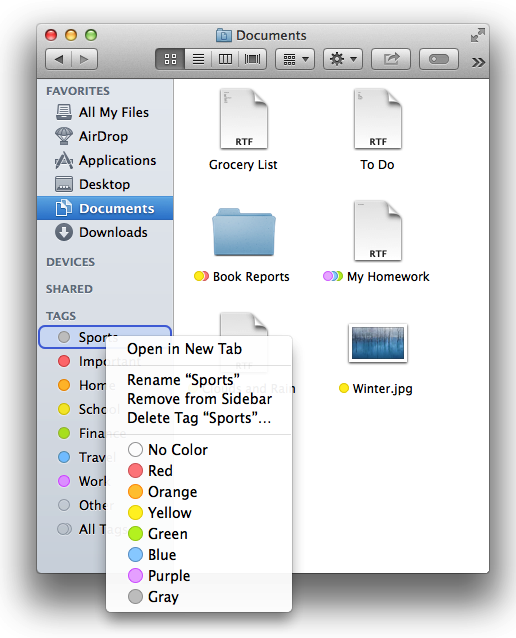
\includegraphics[width=0.8\textwidth]{images/macos_tags.png}
    \end{center}
    \caption{Vue et gestion d'un tag dans le Finder macOS \cite{ref5}}
    \label{macos_tags}
\end{figure}
Lorsque l'on clique sur un tag, une recherche Spotlight est effectuée. Spotlight est le moteur de 
recherche interne à macOS. Spotlight garde un index des tags, fournissant un accès rapide aux 
fichiers correspondants \cite{ref9}.
Tous ces tags peuvent se synchroniser sur les différents "iDevices" via iCloud. Finalement, 
un menu de réglages permet la gestion des tags (affichage, suppression, etc.) \cite{ref5}, 
\cite{ref6}. L'implémentation de ce système utilise les extended attributes (voir section 
\ref{extended_attributes}) pour stocker les tags. Les différents tags se trouvent dans l'attribut 
\mintinline{shell}{kMDItemUserTags}, listés les uns à la suite des autres. Via le Terminal, à 
l'aide de la commande \mintinline{shell}{mdls}, nous pouvons afficher la liste des tags associés à 
un fichier, nommé "Hello" pour l'exemple :
\begin{code}
    \begin{minted}[bgcolor=mygray,breaklines,breaksymbol=,linenos,frame=single,stepnumber=1,tabsize=2]{shell}
% mdls -name kMDItemUserTags Hello 
kMDItemUserTags = (
    Green,
    Red,
    Essential
)
    \end{minted}
    \caption{\mintinline{shell}{mdls} listant les tags d'un fichier sous macOS \cite{ref7}}
\end{code}
\bigbreak
Ici, ce fichier "Hello" est étiqueté avec trois tags, "Green", "Red" et "Essential". Le fait que 
l'indexation est réalisée avec Spotlight implique une réindexation des fichiers dans le cas d'un 
changement de nom pour un tag donné sous macOS. Le framework système \mintinline{text}{FSEvents} 
donne une solution partielle : c'est une API (utilisée également par Spotlight) qui offre aux 
applications la possibilité d'être notifiées si un changement a eu lieu sur un dossier (un événement 
toutes les 30 secondes). \mintinline{text}{FSEvents} maintient des logs de ces changements dans 
des fichiers, les applications peuvent ainsi retrouver l'historique des changements quand elles 
le veulent \cite{ref10}.


\section{Analyse des besoins} %--------------------------------------------------
\cite{ref3}
% surveillance des fichiers
% indexation
% peu de latence
% temps réel
% périph amovible garde index
% rust
% efficace et peu de mémoire
% bcp de fichiers (million)



\section{Technologies} %--------------------------------------------------
\subsection{Rust}
\cite{ref0} \cite{ref1} \cite{ref2}

\subsection{Les extended attributes}\label{extended_attributes}
\subsubsection{Théorie}
Les extended attributes, ou "attributs étendus" en français, sont un moyen d'attacher des 
méta-données aux fichiers et dossiers sous forme de paires \mintinline{text}{espace:nom:valeur}. 
L'espace de nom, ou \textit{namespace} en anglais, définit les différentes classes d'attributs. 
Dans le cadre de ce projet, l'accent est mis sur ext4 sous Linux, il actuellement 4 espaces de noms 
ou classes : \mintinline{text}{user}, \mintinline{text}{trusted}, \mintinline{text}{security} et 
\mintinline{text}{system}. L'espace qui nous intéresse est \mintinline{text}{user}. C'est là que 
l'utilisateur ou l'application, pour autant qu'il ait les droits usuels UNIX sur les fichiers, peut 
manipuler les extended attributes. Les 3 autres espaces de noms sont utilisés entre autres pour 
les listes d'accès ACL (\mintinline{text}{system}), les modules de sécurité du kernel 
(\mintinline{text}{security}) ou par \mintinline{text}{root} (\mintinline{text}{trusted})
\cite{ref11} \cite{ref12}.
Le nom est une chaine de caractères et la valeur peut être une chaine de caractères ou des données binaires. 
Les extended attributes sont stockés dans les fichiers. De nombreux systèmes de fichiers gèrent leur 
usage : ext2-3-4, XFS, Btrfs, UFS1-2, NTFS, HFS+, ZFS. Ces systèmes de fichiers sont utilisés par 
les 4 systèmes d'exploitation les plus répandus : Windows, macOS, Linux et FreeBSD. Windows utilise 
les extended attributes notamment dans sa gestion des permissions Unix dans le shell Linux intégré 
à Windows 10 \cite{ref21}. macOS, comme vu à la section \ref{existant_macOS}, les utilise entre 
autres dans son système de gestion des tags. La commande \mintinline{text}{xattr} permet de les 
manipuler. Sous Linux, il en existe 3 : \mintinline{text}{attr}, \mintinline{text}{getfattr} et 
\mintinline{text}{setfattr}. Sous Linux avec ext2-3-4, chaque attribut dispose d'un bloc de données 
(1024, 2048 ou 4096 bytes) \cite{ref12}.
Apple et freedesktop.org préconisent la notation DNS inversée pour 
nommer les attributs \cite{ref8}, \cite{ref24} car n'importe quel processus peut modifier les 
attributs dans l'espace utilisateur. En préfixant du nom du programme le nom de l'attribut, par 
exemple \mintinline{text}{user.myprogram.myattribute}, on diminue le risque qu'une autre 
application utilise le même nom d'attribut. Malheureusement, la plupart des outils CLI Linux 
pour manipuler les fichiers comme \mintinline{text}{cp}, \mintinline{text}{tar}, etc. ne prennent 
pas en compte les attributs avec leur syntaxe par défaut \cite{ref4}.

\subsubsection{Petites manipulations}
Pour vérifier la portabilité des extended attributes, quelques tests ont été réalisés entre un 
SSD faisant office de disque système à Linux Mint avec 2 clés USB (de 8 et 64 Go) et un emplacement 
réseau monté en NFS. Le listing suivant montre la sortie de la commande \mintinline{bash}{df}, qui 
renvoie l'utilisation des différents emplacements de stockage, dans l'ordre : le disque système, en 
ext4, la clé de 8 Go formatée une fois en FAT32, puis une autre fois en NTFS, la clé de 64 Go formatée 
en ext4 et finalement une machine virtuelle sous Debian 9 montée en NFS.
\bigbreak
\begin{code}
    \begin{minted}[bgcolor=mygray,breaklines,breaksymbol=,linenos,frame=single,stepnumber=1,tabsize=2]{text}
Sys. de fichiers        Type   Taille Utilisé Dispo Uti% Monté sur
/dev/sda2               ext4     451G    334G   96G  78% /
/dev/sdg1               vfat     7.7G    4.0K  7.7G   1% /media/pc/cle1
/dev/sdg1               fuseblk  7.7G     41M  7.7G   1% /media/pc/cle1
/dev/sdg1               ext4      59G     33G   23G  59% /media/pc/cle2
192.168.1.21:/home/user nfs4     916G    198G  673G  23% /mnt/debian
    \end{minted}
    \caption{Output de \mintinline{bash}{df -Th} : le disque système, les clés USB et le NFS}
\end{code}
\bigbreak
La démarche est la suivante : un extended attribute dans l'espace \mintinline{text}{user} avec 
comme nom \mintinline{text}{author} et comme valeur \mintinline{text}{steven} est ajouté au fichier 
\mintinline{text}{file.txt} avec \mintinline{bash}{attr}. Ce fichier est copié avec 
\mintinline{bash}{cp} en prenant garde à préserver l'attribut (option 
\mintinline{bash}{--preserve=xattr}). Une fois copié, on tente de lire le même attribut, toujours 
avec \mintinline{bash}{attr}. Les résultats sont les suivants :
\bigbreak
\begin{code}
    \inputminted[bgcolor=mygray,breaklines,breaksymbol=,linenos,frame=single,stepnumber=1,
        tabsize=2,firstline=45,lastline=49]{text}{text/test_attr.txt}
    \caption{Copie sur clé USB 8 Go, FAT32}
\end{code}
\bigbreak
\begin{code}
    \inputminted[bgcolor=mygray,breaklines,breaksymbol=,linenos,frame=single,stepnumber=1,
        tabsize=2,firstline=54,lastline=61]{text}{text/test_attr.txt}
    \caption{Copie sur clé USB 8 Go, NTFS}
\end{code}
\bigbreak
\begin{code}
    \inputminted[bgcolor=mygray,breaklines,breaksymbol=,linenos,frame=single,stepnumber=1,
        tabsize=2,firstline=66,lastline=73]{text}{text/test_attr.txt}
    \caption{Copie sur clé USB 64 Go, ext4}
\end{code}
\bigbreak
\begin{code}
    \inputminted[bgcolor=mygray,breaklines,breaksymbol=,linenos,frame=single,stepnumber=1,
        tabsize=2,firstline=78,lastline=79]{text}{text/test_attr.txt}
    \caption{Copie sur l'emplacement réseau distant, NFS}
\end{code}
\bigbreak
On constate que l'opération est infructueuse sur la clé en FAT32 et sur l'emplacement réseau monté 
en NFS alors qu'elle réussit sur les clés USB en NTFS et ext4.

\subsection{Notifications}

\section{Indexation}


\section{Architecture} %--------------------------------------------------


\section{Réalisation} %--------------------------------------------------
\subsection{Tag Manager}
La première réalisation de ce projet est un outil en ligne de commande, écrit en Rust, permettant 
de facilement lister, ajouter et supprimer des tags à des fichiers et dossiers. Il fait usage de 
deux \textit{crates} disponibles sur \href{https://crates.io}{crates.io} : clap \cite{ref22} et 
xattr \cite{ref23}. Clap (Command Line Argument Parser for Rust) est une librairie pour parser 
les arguments d'un programme en ligne de commande. Xattr est une API en Rust pour récupérer, lister, 
ajouter/modifier et supprimer des extended attributes avec Rust. Elle fait appel aux appels systèmes 
en C.
% Insérer quelques bouts de code intéressants. -> examples/01a_quick_example.rs pour clap
% Insérer capture/exemple d'utilisation

\section{Discussion/résultats} %--------------------------------------------------
% cahier des charges rempli ?
% réalisation OK ?
% performances
% Rust VS C
% Bugs
% Améliorations futures



\section{Conclusion} %--------------------------------------------------
\subsection{Remerciements}


\newpage
\section{Références} %--------------------------------------------------
\bibliographystyle{unsrt}
\bibliography{bib}

\end{document}

% \begin{figure}
%     \begin{center}
%         \includegraphics[width=0.8\textwidth]{images/image.png}
%     \end{center}
%     \caption{légende}
%     \label{label}
% \end{figure}

% \begin{code}
%     \begin{minted}[bgcolor=mygray,breaklines,breaksymbol=,linenos,frame=single,stepnumber=1,tabsize=2]{rust}
% fn main() {
%     println!("Hello, world!");
% }
%     \end{minted}
%     \caption{Hello world en Rust}
% \end{code}
% \bigbreak

% \begin{code}
%     \inputminted[bgcolor=mygray,breaklines,breaksymbol=,linenos,frame=single,stepnumber=1,
%         tabsize=2,firstline=157,lastline=185]{rust}{file.rs}
%     \caption{légende}
% \end{code}
% \bigbreak
